\documentclass{article}
\usepackage{pgfplots}
\usepackage{siunitx}
\usepackage[paperheight=2.9in,paperwidth=3.9in,margin=0in]{geometry}
\pgfplotsset{compat=1.17}
\usepgfplotslibrary{external}
\usepgfplotslibrary{fillbetween}

\tikzexternalize

\definecolor{pastelred}{rgb}{1.0, 0.41, 0.38}
\definecolor{pastelmagenta}{rgb}{0.96, 0.6, 0.76}\definecolor{pastelpink}{rgb}{1.0, 0.82, 0.86}

\begin{document}
 \pagenumbering{gobble} 
\pgfplotsset{every axis plot/.append style={line width=1pt, font=\large,}}
\tikzsetnextfilename{test.pdf}

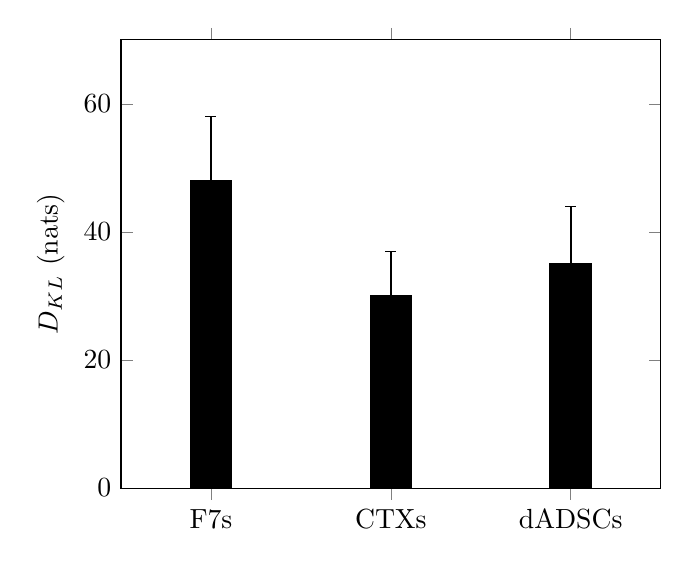
\begin{tikzpicture}
    \begin{axis}[
        ybar,
        bar shift=0pt,
        bar width=15pt,
        ylabel = {$D_{KL}$ (nats)},
        xmin=-0.1,
        xmax=2.9,
        xtick={0.4,1.4,2.4},
        xticklabels={F7s,CTXs,dADSCs},
        scaled y ticks = false,
        ymin=0, ymax=70,
    ]
        \addplot[ybar, fill=black, error bars/.cd,y dir=both,y explicit, error bar style={thick}] coordinates {(0.4,48)+- (0.5,10)};
        
        \addplot[ybar, fill=black, error bars/.cd,y dir=both,y explicit, error bar style={thick}] coordinates {(1.4,30)+- (1.5,7)};  
        
        \addplot[ybar, fill=black, error bars/.cd,y dir=both,y explicit, error bar style={thick}] coordinates {(2.4,35)+-(2.5,9)};


    \end{axis}
\end{tikzpicture}
\end{document}

